\chapter{Virheiden havaitseminen}

\section{Virheiden havaitseminen}

Kenties tärkein staattisen tyyppijärjestelmän tehtävä on havaita ja estää
ohjelmoijan virheitä. Tässä esitellyt työkalut, mahdollisesti Closure
kääntäjää lukuunottamatta, onkin kehitetty erityisesti tätä tarkoitusta
varten.

Kaikki kolme työkalua antaisivat käännösvirheen jos esimerkeissä
\ref{lst:ostoskorin_hinta_clojure} ja \ref{lst:ostoskorin_hinta_flow}
esiteltyä funktiota kutsuttaisiin virheellisesti esimerkiksi listalla
hintaa kuvaavia numeroita, sillä funktion parametrin on annotoitu olevan
lista ``Ostos''-tyyppimääritelmän mukaisia objekteja. Esimerkiksi
virheellinen kutsu
\colorbox{lightgray}{\lstinline|ostoskorinHinta([5, 10, 15])|} ei itse
asiassa aiheuttaisi suoritettaessa ohjelman keskeyttävää virhettä.
\colorbox{lightgray}{\lstinline|ostos.hinta|} ilmaisu on sallittu vaikka
muuttuja \colorbox{lightgray}{\lstinline|ostos|} olisikin arvoltaan numero
eikä objekti. Tällöin ilmaisun arvo on \colorbox{lightgray}{\lstinline|undefined|}
ja lausekkeen \colorbox{lightgray}{\lstinline|summa += ostos.hinta|} jälkeen
\colorbox{lightgray}{\lstinline|summa|} muuttujan arvo on erityinen
ei-numeroa kuvaava \colorbox{lightgray}{\lstinline|NaN|} \cite{Ecma262NaN}.
Käännösaikaisen tarkistamisen merkitys korostuu erityisen hyödylliseksi
tämänkaltaisen ohjelmointivirheen kohdalla, sillä virhe ei välttämättä ole
muutoin helposti havaittavissa. Funktiokutsu ei aiheuttaisi helposti
todennettavaa suoritusaikaista virhettä, joten ei-toivottu palautusarvo
\colorbox{lightgray}{\lstinline|NaN|} saattaisi kiertää ohjelman
operaatioiden välillä pitkällekin aiheuttaen muita loogisia virheitä.

Vuonna 2017 tehdyssä tutkimuksessa TypeScriptin ja Flown vaikutuksesta avoimen
lähdekoodin JavaScript-projekteihin havaittiin, että vähintään 15\%
ilmoitetuista ja korjatuista bugeista olisi voitu havaita ja välttää jos
projektin kehitykseen oltaisin käytetty jompaakumpaa näistä työkaluista \cite{ToTypeOrNotToType}.
To Type or Not to Type: Quantifying Detectable Bugs in JavaScript -tutkimuksen
arvioinnissa huomioitiin lisäksi, että tulos on tutkimusmenetelmästä
johtuen mitä luultavimmin alempi kuin tällaisen muutoksen tuoma todellinen
vaikutus. Tutkimus toteutettiin muuntamalla avoimen lähdekoodin
JavaScript-kirjastoja ensin staattisesti tyypitettyyn muotoon ja sitten
testaamalla kuinka hyvin tyyppitarkastus havaitsi ennalta tunnettuja bugeja
aiheuttavan koodin. Sen ulkopuolelle jäivät bugit joita ei oltu vielä
korjattu tai havaittu, sekä bugit jotka kehittäjä oli havainnut jossain
kehitysvaiheessa ennen virheellisen ohjelman julkaisua. Staattisen
tyyppitarkastus luultavasti auttaisi vähentämään myös näitä bugeja.

\begin{figure}
\centering
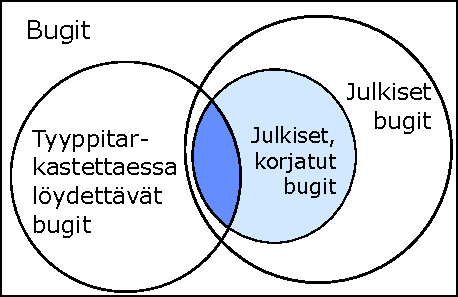
\includegraphics{images/to_type_or_not_to_type_venn.pdf}
\caption{To Type or Not to Type: Quantifying Detectable Bugs in JavaScript
         -tutkimuksen käsittelemät bugit\cite{ToTypeOrNotToType}.}
\label{fig:ToTypeOrNotToType}
\end{figure}

Kuvaajan \ref{fig:ToTypeOrNotToType} esittämässä tilanteessa suuri osa
bugeista ei ole julkisia, eli kehittäjät eivät ole havainneet bugia eivätkä
käyttäjät ole ilmoittaneet sellaisesta. Esimerkiksi seuraavanlainen koodi
saattaisi aiheuttaa vaikeasti havaittavan virheen, joka jäisi dynaamisessa
testaamisessa huomaamatta:

\begin{minipage}{\linewidth}
\begin{lstlisting}[caption={Vaikeasti havaittavan virheen aiheuttava koodiesimerkki}]
if (viikonpaiva === "perjantai") {
  // Alennus perjantaisin 5 euroa
  ostoskori.lisaaTuote({ nimi: "astiasto", Hinta: 10 });
} else {
  ostoskori.lisaaTuote({ nimi: "astiasto", hinta: 15 });
}
\end{lstlisting}
\end{minipage}
Esimerkin koodi ei toimi oikein perjantaisin, sillä \inlinecode{Ostos}-tyyppisen
objektin ominaisuus \inlinecode{hinta} on virheellisesti kirjoitettu isolla
alkukirjaimella. Koska bugi toistuu vain tietyissä olosuhteissa, se voi pysyä
havaitsemattomana pitkään. Staattiselle analyysille konditionaalisen ohjelman
tarkistaminen ei kuitenkaan ole ongelma ja tyyppiannotoituna kaikki kolme
työkalua pystyvätkin osoittamaan esimerkissä olevan virheen.

\section{Ohjelman optimointi käännösvaiheessa}
TODO

\section{Tyyppimäärittelyt dokumentaationa}
TODO